\section{Datasample, Event Selection, and Noise Cleaning} \label{sec:EventSelection}

{\bf Dataset and CMSSW release:}
\begin{itemize}
\item dataset: /MinimumBias/Commissioning10-GOODCOLL-Jun9thSkim\_v1/RECO
\item CMSSW release: CMSSW\_3\_7\_0\_patch2
\end{itemize}

{\bf Event selection:}
\begin{itemize}
\item Physics declared bit
\item BPTX bit 0
\item Removal of beam scraping events
\item Good primary vertex
\item Good Run/LS selection. JSON file: Cert\_132440-136119\_7TeV\_May27thReReco\_Collisions10\_JSON.txt  
\end{itemize}
More details at [XXX].

{\bf Noise cleaning}

Noise cleaning/event filter for calotower-based $\etmiss$ algorithms (Calo$\etmiss$ and tc$\etmiss$):
\begin{itemize}
\item ECAL barrel spikes (reject RecHits): topology (kWeird flag = swiss cross variable) + timing (kOutOfTime flag) [XXX];
\item HF PMT hits (reject Rechits): topology (HFLongShort flag = PET+S9/S1) + pulse shape (HFDigiTime flag) [XXX];
\item HPD/RBX noise in HBHE (reject events): combination of pulse shape and topological variables [XXX].
\end{itemize}

Noise cleaning (reject RecHits) for pf$\etmiss$ is described at [XXX]. Timing and topology are used to reject RecHits 
affected by ECAL and HF noise. Topology only is used to reject rechits affected by HBHE noise. No events are rejected.

NOTE: The HPD/RBX noise filter is applied for both the tc$\etmiss$ and pf$\etmiss$ analysis presented in this note, 
in order to have the same number of events passing the selection.

%Figure~\ref{fig:calomet} shows the cleaned Calo$\etmiss$ distribution for $\approx 19.6$~M events 
%passing the event selection described above.
%\begin{figure}[h]
% \centering
% \begin{tabular}{ll}
%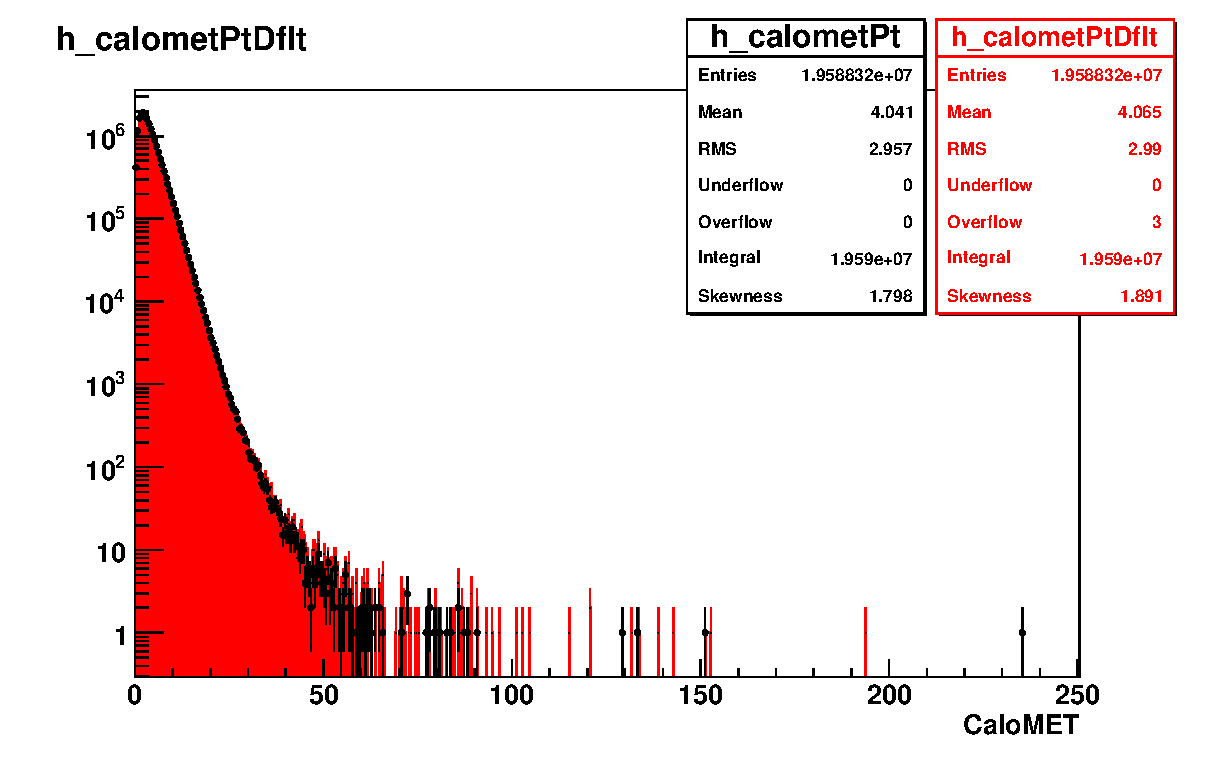
\includegraphics[width=0.7\textwidth]{fig/calomet.eps} 
% \end{tabular}
%\caption{Calo$\etmiss$ distribution of 7 TeV collision data after applying the event selection described
%in this section. Red filled histogram is obtained using the $\etmiss$ value coming from default CMS reconstruction 
%in CMSSW\_358p3. The black dotted histogram is the $\etmiss$ after applying the full noise cleaning 
%procedure described in this section.}
%\label{fig:calomet}
%\end{figure}